\documentclass[
    german=false,
    thesistype=dissertation,
    nolistoffigures,
    nolistoftables,
]{tubsthesis}

\usepackage{lipsum}

\thesisname{Johanna Doe}
\thesismatrikel{1234567}
\thesisemail{j.doe@tu-braunschweig.de}
\thesismajor{Informatik}
\thesisduration{3}
\thesissupervisors{Super Visor, M. Sc.}{Dr. Dipper Visor}{}
\thesisprofessor[Prof.\,Dr.-Ing.\,Jane Smith]{Prof.\,Dr.-Ing.\,Lars Eisbär}
\thesistitle{Titel der Thesis}{Title of the thesis}
\thesisbegindate{2020-01-01}
%\thesisenddate{2020-01-02}
\thesispresentationpoints{5.7}

\addbibresource{bibliography.bib}

\thesisinstitute{Institute of Perfect Writing in IT}
\thesisbirthdate{2020-05-28}
\thesisbirthplace{Braunschweig}
\thesisfaculty{Carl-Friedrich-Gauß-Fakultät}
\thesisdegree[einer]{Doktoringenieurin (Dr.-Ing.)}
\titlepicture{images/infozentrum.jpg}

\begin{document}
    \thesisabstract[%
        This is an english text.\\
        \lipsum[1-2]
    ]{%
        Hier steht ein Text auf Deutsch.\\
        \lipsum[3-4]
    }
    
    \thesisposttitle{
        \clearpage
        \section*{What I've always wanted to add after the title page...}
        Thank you
        \section*{Acknowledgments}
        \lipsum[5-6]
    }
    
    \begin{thesis}

        \chapter{Intro}

        \lipsum[1-3]

        \begin{figure}
        \centering
        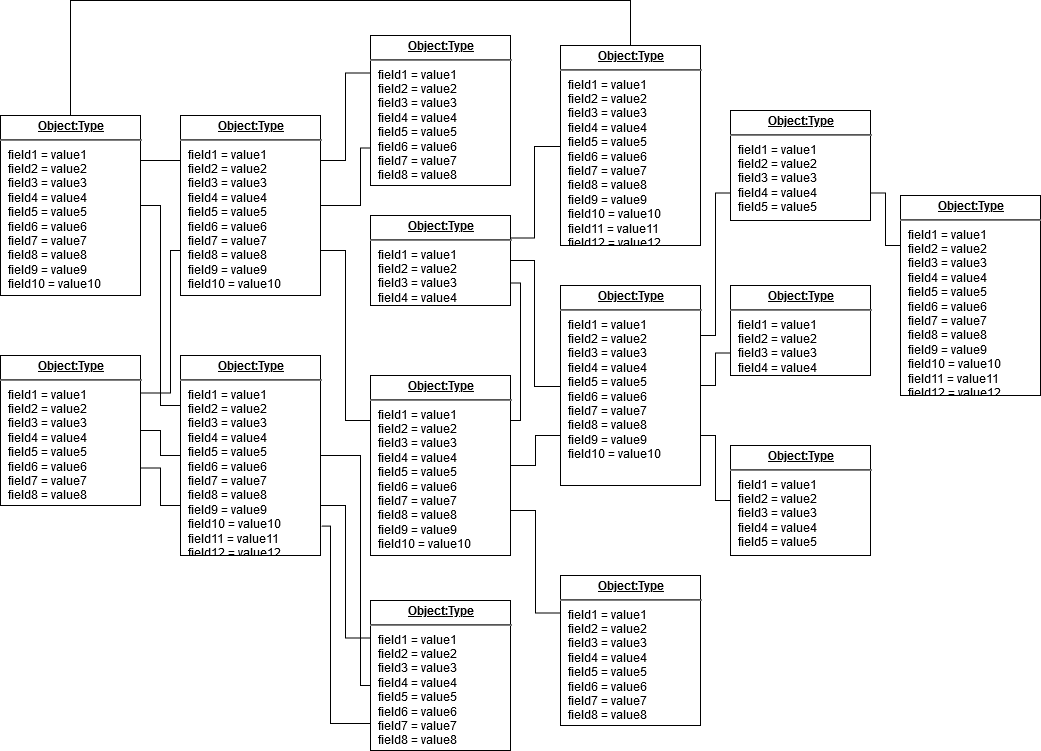
\includegraphics[width=\textwidth]{images/example_diagram.png}
        \caption{Some diagram, not relevant to anything~\cite{lisa}}
        \label{fig:inga}
        \end{figure}

        \lipsum[4-7]

    \end{thesis}

    \chapter{Storage Device}
    Put a table of the contents of your attached Storage Device (SD card/USB flash drive) here.
    Add explanations where needed!
\end{document}